\documentclass[border=10pt]{standalone}
\usepackage[svgnames]{xcolor}
\usepackage{amsmath}
\usepackage{pgfplots}
\pgfplotsset{compat=newest}
\usepackage[sfdefault]{FiraSans}
\usepackage{FiraMono}
\renewcommand*\familydefault{\sfdefault}
\begin{document}
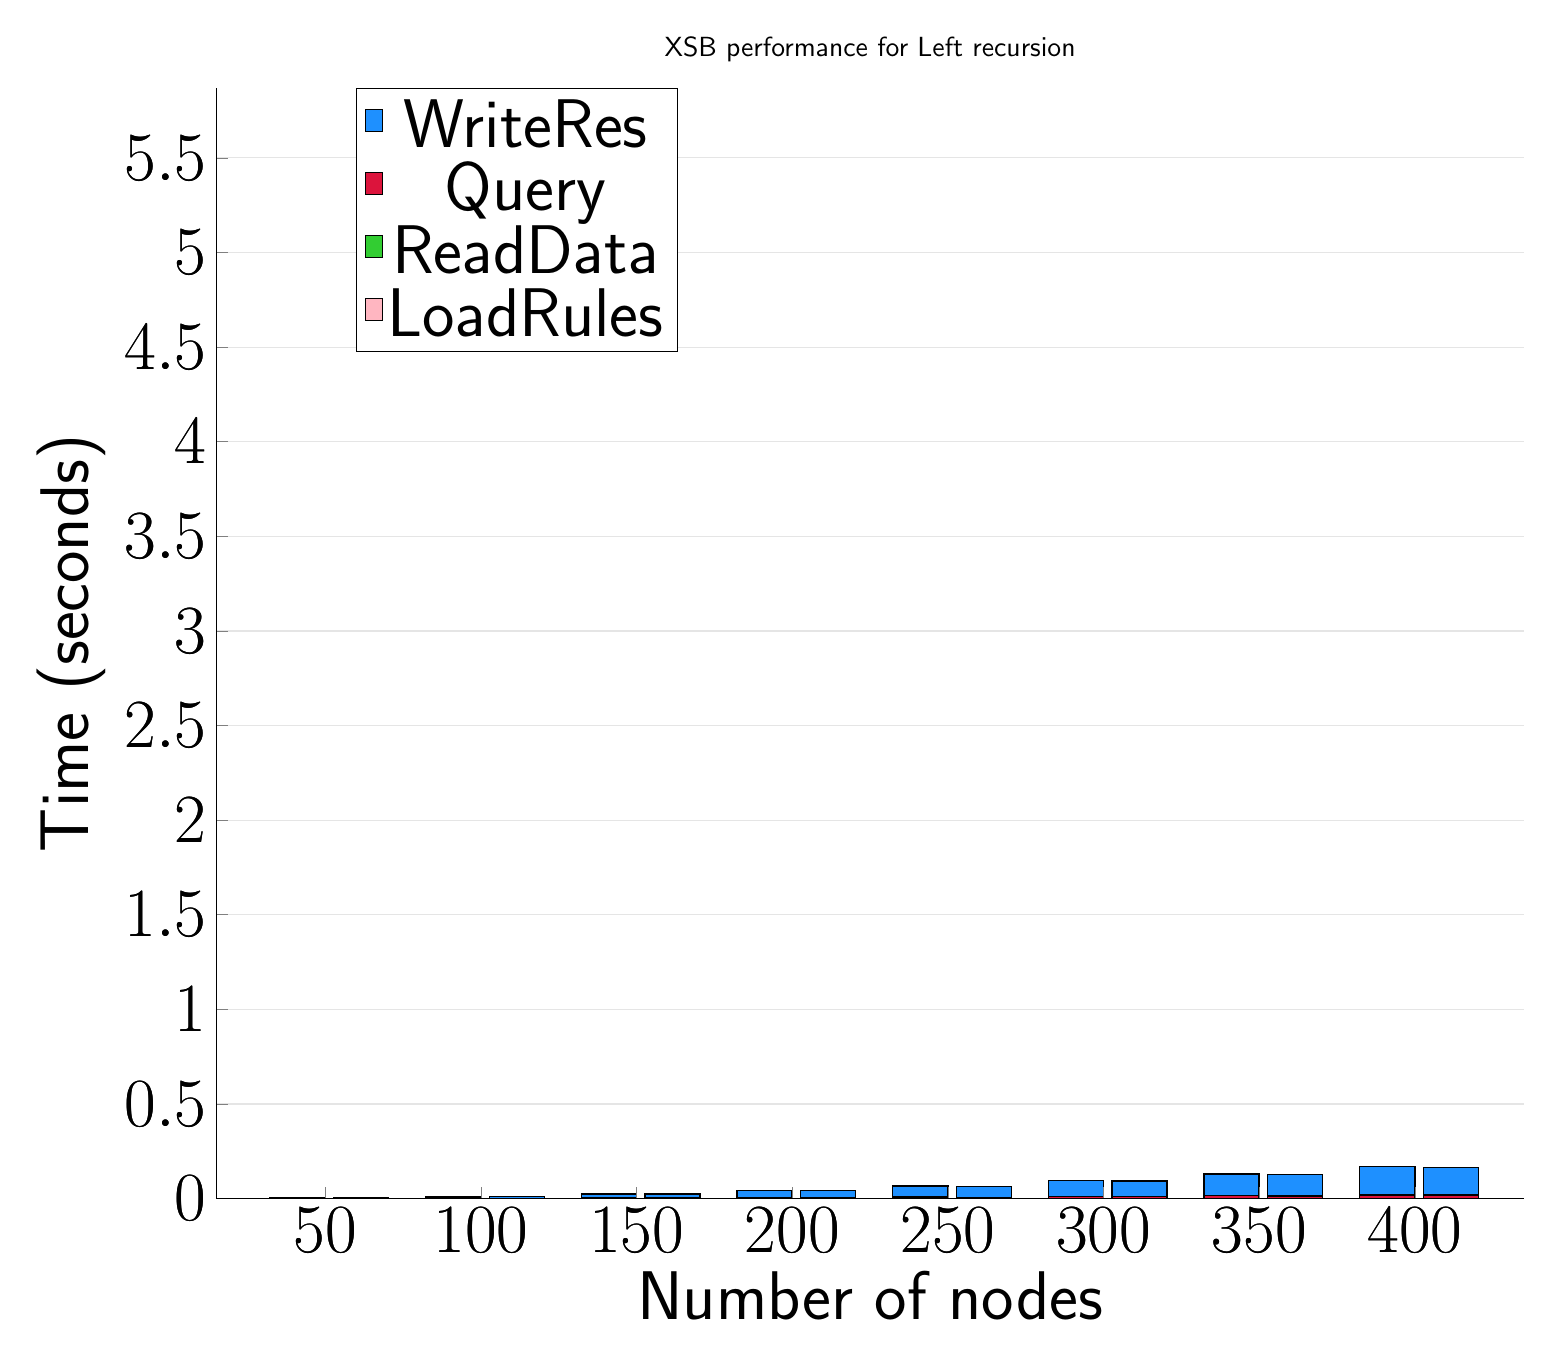
\begin{tikzpicture}
	\begin{axis}[
			ybar stacked,
			title={XSB performance for Left recursion},
			bar shift=-10pt,
			width=1.5\textwidth,
			bar width=0.7cm,
			ymajorgrids, tick align=inside,
			major grid style={draw=gray!20},
			xtick=data,
			ymin=0, ymax=5.870271515846253,
			axis x line*=bottom,
			axis y line*=left,
			enlarge x limits=0.1,
			legend style={
					at={(0.23, 1)},
					anchor=north,
					legend columns=1,
					font=\Huge,
				},
			ylabel={Time (seconds)},
			xlabel={Number of nodes},
			label style={font=\Huge},
			tick label style={font=\Huge},
		]
		\addlegendimage{fill=DodgerBlue, draw=black, line width=0.2pt}
		\addlegendentry{WriteRes}
		\addlegendimage{fill=Crimson, draw=black, line width=0.2pt}
		\addlegendentry{Query}
		\addlegendimage{fill=LimeGreen, draw=black, line width=0.2pt}
		\addlegendentry{ReadData}
		\addlegendimage{fill=LightPink, draw=black, line width=0.2pt}
		\addlegendentry{LoadRules}
		\addplot +[fill=LightPink, draw=black, line width=0.5pt] coordinates {
				(50, 0.001097249984741211)
				(100, 0.00104081630706787)
				(150, 0.001103782653808595)
				(200, 0.0010551691055297858)
				(250, 0.001030707359313966)
				(300, 0.0010808467864990231)
				(350, 0.0010599136352539061)
				(400, 0.0010618925094604491)
			};
		\addplot +[fill=LimeGreen, draw=black, line width=0.5pt] coordinates {
				(50, 0.0003676891326904295)
				(100, 0.00042967796325683595)
				(150, 0.0004860162734985353)
				(200, 0.000522613525390625)
				(250, 0.0005663394927978517)
				(300, 0.0005985975265502929)
				(350, 0.0006633758544921876)
				(400, 0.0007078409194946288)
			};
		\addplot +[fill=Crimson, draw=black, line width=0.5pt] coordinates {
				(50, 0.0002557516098022461)
				(100, 0.0010059118270874029)
				(150, 0.0023272752761840836)
				(200, 0.004007816314697266)
				(250, 0.006232810020446777)
				(300, 0.009386229515075683)
				(350, 0.0137094497680664)
				(400, 0.01777923107147216)
			};
		\addplot +[fill=DodgerBlue, draw=black, line width=0.5pt] coordinates {
				(50, 0.0025915145874023425)
				(100, 0.009669089317321779)
				(150, 0.02126986980438233)
				(200, 0.03790814876556397)
				(250, 0.0587409496307373)
				(300, 0.08479301929473877)
				(350, 0.11456794738769523)
				(400, 0.14913334846496584)
			};
	\end{axis}
	\begin{axis}[
			ybar stacked,
			bar shift=13pt,
			width=1.5\textwidth,
			bar width=0.7cm,
			ymajorgrids, tick align=inside,
			major grid style={draw=none},
			xtick=data,
			ymin=0, ymax=5.870271515846253,
			axis x line*=none,
			axis y line*=none,
			enlarge x limits=0.1,
			label style={font=\Huge},
			tick label style={font=\Huge},
		]
		\addplot +[fill=LightPink, draw=black, line width=0.5pt] coordinates {
				(50, 0.0006176)
				(100, 0.0006015000000000004)
				(150, 0.0006180000000000003)
				(200, 0.0006121000000000002)
				(250, 0.0005969)
				(300, 0.0006033)
				(350, 0.0006004999999999998)
				(400, 0.0006014)
			};
		\addplot +[fill=LimeGreen, draw=black, line width=0.5pt] coordinates {
				(50, 0.0001775000000000002)
				(100, 0.0002229999999999999)
				(150, 0.0002735999999999999)
				(200, 0.0003069999999999998)
				(250, 0.0003516000000000004)
				(300, 0.00038649999999999996)
				(350, 0.0004424999999999999)
				(400, 0.0004886000000000001)
			};
		\addplot +[fill=Crimson, draw=black, line width=0.5pt] coordinates {
				(50, 0.00024080000000000008)
				(100, 0.0009566000000000005)
				(150, 0.0022169)
				(200, 0.0038367000000000006)
				(250, 0.005970500000000001)
				(300, 0.0089801)
				(350, 0.013168700000000002)
				(400, 0.017085299999999998)
			};
		\addplot +[fill=DodgerBlue, draw=black, line width=0.5pt] coordinates {
				(50, 0.0023085000000000002)
				(100, 0.009261599999999998)
				(150, 0.0206914)
				(200, 0.0369655)
				(250, 0.05706019999999999)
				(300, 0.083223)
				(350, 0.1125246)
				(400, 0.1459568)
			};
	\end{axis}
\end{tikzpicture}

\end{document}
